\documentclass[12pt]{article}
    % General document formatting
    \usepackage{geometry}
    \geometry{
    left=1.5in,
    top=1in,
    right=1in,
    bottom=1in
    }
    \usepackage{apacite}
    \usepackage{pdfpages}
    \usepackage[parfill]{parskip}
    \usepackage{amsopn}
    \usepackage{todonotes}
    \usepackage{mathtools}
    \usepackage[utf8]{inputenc}
    \usepackage{multicol}
    \usepackage{amsmath,amssymb,amsfonts,amsthm}
    \usepackage{dot2texi}
    \usepackage{tikz}
    \usepackage{mdframed}
    \usepackage[section]{placeins}
    \usepackage{mathptmx}
    \usepackage{sectsty}
    \usepackage{fancyhdr}
    % \usepackage{hyperref}
    % \usepackage[figure]{hypcap}

    \makeatletter
    \renewcommand{\section}{\@startsection
    {section}%                   % the name
    {1}%                         % the level
    {\z@}%                       % the indent / 0mm
    {-\baselineskip}%            % the before skip / -3.5ex \@plus -1ex \@minus -.2ex
    {0.5\baselineskip}%          % the after skip / 2.3ex \@plus .2ex
    {\centering\large\bfseries\MakeUppercase}} % the style
            
    \usetikzlibrary{shapes,arrows}

    \DeclareMathOperator{\StringT}{StringT}
    \DeclareMathOperator{\NumberT}{NumberT}
    \DeclareMathOperator{\BooleanT}{BooleanT}
    \DeclareMathOperator{\LitT}{LitT}
    \DeclareMathOperator{\JSLit}{\textit{JSLit}}
    \DeclareMathOperator{\JSTypeof}{JSTypeof}
    \DeclareMathOperator{\RecT}{RecT_\Gamma}
    \DeclareMathOperator{\ObjT}{ObjT_\Gamma}
    \DeclareMathOperator{\ListT}{ListT_\Gamma}
    \DeclareMathOperator{\SetT}{SetT_\Gamma}
    \DeclareMathOperator{\MapT}{MapT_\Gamma}
    \DeclareMathOperator{\ObjType}{ObjType}
    \DeclareMathOperator{\UnionT}{UnionT_\Gamma}
    \DeclareMathOperator{\InterT}{InterT_\Gamma}
    \DeclareMathOperator{\LookupObjRef}{\Gamma}
    \DeclareMathOperator{\Identifier}{\textit{Identifier}}
    \DeclareMathOperator{\Number}{Number}
    \DeclareMathOperator{\Boolean}{Boolean}
    \DeclareMathOperator{\type-ref}{ref}
    \DeclareMathOperator{\Type}{{\textit{Type}_\Gamma}}
    \DeclareMathOperator{\NoSuper}{NoSuper}
    \DeclareMathOperator{\InterOrObj}{InterOrObj}
    \DeclareMathOperator{\ObjectSubtype}{ObjectSubtype_\Gamma}
    \DeclareMathOperator{\RecordSubtype}{RecordSubtype}
    \DeclareMathOperator{\Value}{Value_{\Gamma, \Sigma}}
    \DeclareMathOperator{\IdentifierV}{StringV}
    \DeclareMathOperator{\NumberV}{NumberV}
    \DeclareMathOperator{\BooleanV}{BooleanV}
    \DeclareMathOperator{\RecV}{RecV_{\Gamma, \Sigma}}
    \DeclareMathOperator{\ObjV}{ObjV_{\Gamma, \Sigma}}
    \DeclareMathOperator{\ListV}{ListV_{\Gamma, \Sigma}}
    \DeclareMathOperator{\SetV}{SetV_{\Gamma, \Sigma}}
    \DeclareMathOperator{\MapV}{MapV_{\Gamma, \Sigma}}
    \DeclareMathOperator{\UnionV}{UnionV_{\Gamma, \Sigma}}
    \DeclareMathOperator{\ValueType}{ValueType_{\Gamma, \Sigma}}
    \DeclareMathOperator{\textref}{ref}
    \DeclareMathOperator{\ObjFields}{ObjFields}
    \DeclareMathOperator{\ObjPairsMatch}{ObjPairsMatch}
    \DeclareMathOperator{\where}{ where }
    \DeclareMathOperator{\textif}{ if }
    \DeclareMathOperator{\suchthat}{s.t.}
    \newcommand{\ValueRef}{\textref}
    \newcommand{\ValueDeref}[1]{\Sigma(#1)}
    \newcommand{\subtype}{<:_\Gamma}

    \newcommand{\href}[2]{\textbf{#2}}

    \setcounter{secnumdepth}{0}
    \linespread{2}
\begin{document}

\title{Sinap's Type System}
\author{Sheyne Anderson}
\renewcommand{\thepage}{\roman{page}}
\let\oldtodo\todo
\renewcommand{\todo}[1]{\oldtodo[inline]{#1}}

\includepdf[fitpaper=true, pages=1]{honorsstuff.pdf}

\section{ABSTRACT}

For the graph program editor Sinap IDE it was necessary to design 
a language (Sinap's Type System) to generically describe families of 
cyclic data structures. The Type System consists pair of languages:
one for describing data and another for describing valid structures
for that data. These two languages are analogous to XML and XML Schema
\cite{Thompson:12:WXS}.

\newpage

\tableofcontents
\todo{remove the todolist}
\listoftodos
\newpage
\setcounter{page}{1}
\renewcommand{\headrulewidth}{0pt}
\pagestyle{fancy}
\fancyhead[R]{\thepage}
\renewcommand{\thepage}{\arabic{page}}
\section{INTRODUCTION}


Graphs are ubiquitous in computer science. They are used
in various data structures to store information, in compiler 
design to describe the structure of programs, and anywhere 
in which one might need to reason about the connections 
in a complicated system. In computation theory, graphs are 
used to describe the various models of computation such as
Deterministic Finite-State Automata (DFAs), Push Down
Automata (PDAs), and Turing Machines. 

When studying these formalisms, it is helpful 
to have an editor to create instances of these various models
and execute them on various inputs. One such editor, 
JFLAP \cite{jflap:book} is used at the University of Utah 
in CS 3100: Models of Computation. JFLAP has several drawbacks
including having a unintuitive user interface, 
being difficult to maintain, and having some bugs 
\cite{jflap:challenges}. We set out to create an editor 
for programming languages that could be depicted visually as 
graphs. These include languages such DFAs, PDAs, and Turing 
Machines, but also neural network models and some general purpose
programming languages such as LabVIEW \cite{Johnson:1997:LGP:541144}.

\subsection{Sinap IDE}

\todo{Our description of Sinap on our website is fairly good, can 
I just quote it in its entirety?}
From \href{https://2graphic.github.io}{2graphic.github.io}:

\todo{just paraphrase the following}

\begin{quotation}
    The goal of Sinap is to provide a generic UI platform 
    for editing and interpreting domain-specific graph-based languages. What does 
    this mean? Let's break it down. Users of Sinap want to design visual 
    representations of state machines or other conceptual tools that can be modeled
    with nodes and edges but don't want to have to create their own UI to handle all
    the fancy drawing stuff. Sinap IDE will provide the heavy lifting for presenting
    the visual side of creating graphs as well as running interpreters for them.
    Where do these interpreters come from? Plugins. Sinap IDE will expose an API
    that developers can use to create their own domain-specific interpreters of
    languages that can be modeled with graphs. These plugins can then be installed
    into Sinap, giving the IDE more power.

    There are many options for graph editors available, but the vast majority of them
    are designed specifically for their respective domains. Sinap IDE aims to break 
    this trend by allowing developers implement their own interpreters that can be 
    used in the application. Think of a lightweight text editor for writing code but 
    replace ``text" with ``graph" and add interpreting and that is what Sinap aims to 
    be. What do we mean by ``interpret"? Sinap is not a tool for simple chart designs. 
    The idea behind Sinap plugins is to be able to feed graphs some input in order to 
    see what the graph produces. Imagine a tool that allows you to step through a state 
    machine that you designed for a project. With Sinap this is possible.
\end{quotation}

While I was involved with the project as a whole, architecting 
data-flow throughout the application, building the interpreters
for the stock plugins, setting up automatic testing, continuous 
intergration, and builds, and generally quashing bugs throughout
the application, my main focus was on the Type System. 

\todo{flow/edit the following}

Sinap IDE is an integrated development environment for various 
graph programing languages. Each of these 
languages is loaded into Sinap as a ``plugin" and is 
referred to as an interpreter (since it runs programs dynamically). 
More information 
about the editor can be found at 
\href{https://2graphic.github.io}{2graphic.github.io}.
Because our goal for Sinap IDE is to be an editor for many 
different graph programming languages, we designed the user interface (UI)
to adapt to best support whichever plugin that is currently loaded. 

While editing a graph, components of the
graph will have different attributes associated with them 
that the editor should present contextually. For example, in
a graph-language describing deterministic finite-state 
automata (DFAs) edges should have a ``symbol" attribute of 
type \texttt{character} corresponding to the input by which this 
edge should be followed. 

\begin{figure}
    % \capstart
    \centering
    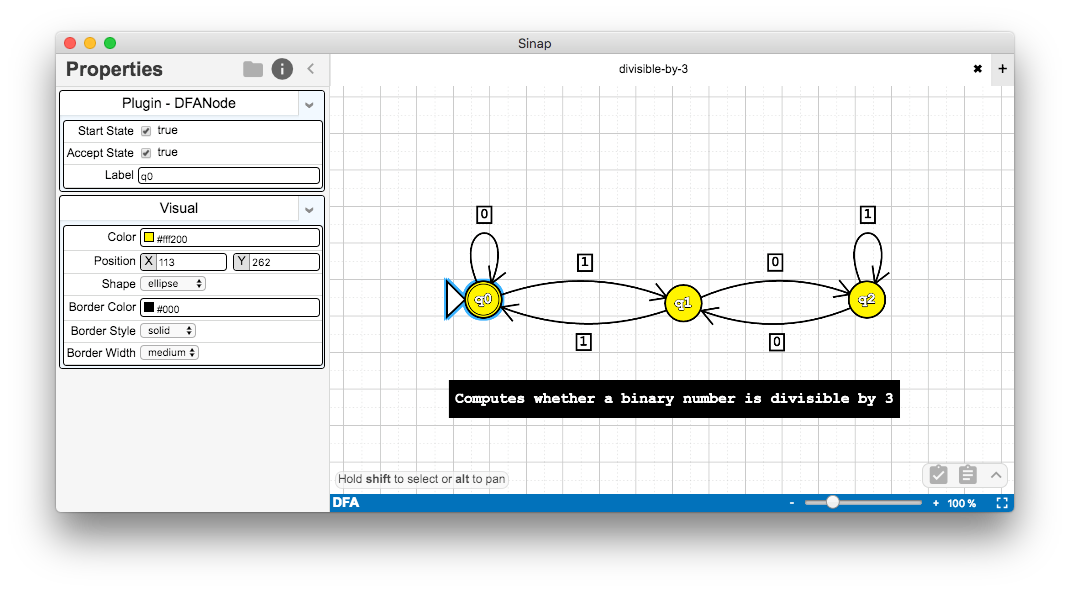
\includegraphics[width=.8\textwidth]{sinap-screenshot}
    \caption{Sinap IDE editing a graph}
    \label{sinap-screenshot}  
\end{figure}

In Figure \ref{sinap-screenshot}, Sinap's UI
presents the user with nodes and edges which can be selected 
and edited in the sidebar. Allowing the sidebar and other UI components to change based
on which interpreter is loaded is the purpose of Sinap's Type System. 
This document presents a model for the type system. 
    
Sinap's Type System consists of two parts:

\begin{enumerate}
    \item A data-language to describe graph components 
    (implemented in values.ts)
    \item A data-description language to define valid schema 
    (implemented in types.ts)
    for the data language
\end{enumerate}

The code for both can be found at 
\href{https://github.com/2graphic/sinap-types}
{github.com/2graphic/sinap-types}.

The data that are allowable in the sidebar can be more complicated than
simple strings and numbers. In Figure \ref{sinap-screenshot}, the ``Position" attribute
of the node has a structure similar to the following TypeScript code:

\vspace{1ex}

\linespread{1}
\begin{verbatim}
type Point = {
    x: number;
    y: number;
}
\end{verbatim}

Complex types aren't limited to fields directly on nodes and edges,
and can be arbitrarily nested. 

The goal of creating Sinap's Type System is to allow plugin/interpreter
implementers to specify what 
kinds of graphs are valid for their interpreter. This means that 
the interpreter specifies the various fields on nodes and edges 
and can assume that those fields are present on all of the graph elements
that it receives. The Type System also allows different kinds of nodes and 
edges to exist in the same graph and allows for rules defining what kinds of
nodes can connect to which edges. 

\todo{``The model is going to be next''}


\section{BACKGROUND}

For many programming languages the only specification for 
semantics if the reference implementation of the interpreter or compiler. 
Python for example specifies valid behavior based on the behavior of the
CPython interpreter \cite{cpython}. Other languages, such as 
C and C++ have an enormous formal document specifying the semantics
of the language. 

For studying a language academically, it is useful to create a model
of a language \cite{redexbook}.

\todo{CONTINUE HERE}


Featherweight Java
Lua
Standard ML


\section{TYPES}

\subsection{Notation}

The symbol \((\operatorname{Kind}_1, ...)\) is equivalent to 
\((\operatorname{Kind}_i)\). They are also equivalent to 
\((\operatorname{Kind}_1, ..., \operatorname{Kind}_n)\)
where \(n\) is unspecified and represent an ordered list 
of \(n\) elements. \(\{\operatorname{Kind}_i\}\) represents 
the set of the elements of the list. 

``\(\_\)'' represents a symbol that has been omitted for brevity.

\subsection{Type Model}
\begin{figure}
    % \capstart
    \begin{mdframed}    
    \begin{multicols}{2}
    
    \begin{verbatim}
    class Node1 {
        label: string;
        customAttribute: number;
    }
    class Node2 {
        label: string;
        otherAttribute: {
            f1: boolean,
            f2: number
        };
    }
    class Edge {
        label: string
        source: Node1;
        destination: Node2;
    }
    type Nodes = Node1 | Node2;
    type Edges = Edge;

    
    
    \end{verbatim}
    \end{multicols}
    \end{mdframed}
    \caption{TypeScript code to go with Figure \ref{types-example}}
    \label{types-example-code}
\end{figure}    

The type system is designed to describe families of valid graphs. 
This is why it ends up looking like the type system of a programming 
language: both solve the problem of describing how data is structured.
An example to motivate Sinap's Type System is given in Figure 
\ref{types-example-code}. Here I show the description of a graph-language
given in TypeScript. There are two types of nodes because 
in general graph languages can have different kinds of nodes in them. 
For example, in a language describing artificial neural networks, 
there might be a convolutional layers, fully connected layers, and 
dropout layers as node types. Sinap Types also supports having multiple
kinds of edges. 

The model for types is composed of two parts. The first is the 
specific representation of types given in Figure 
\ref{sinap-types-model}. The second part defines a subtype
relations on these types and is given in Figure \ref{subtype-definitions}.

Before diving into Figure \ref{sinap-types-model} and 
a formal representation of each of the types, here is a presentation 
of the various types with descriptions in english. 
\begin{itemize}
    \item \(\StringT\) is a type representing all strings.
    \item \(\NumberT\) is a type representing all numbers.
    \item \(\BooleanT\) is a type representing all booleans.
    \item \(\LitT(\JSLit)\) is the type for literal primitives, specifically,
    string, number, and boolean literals. 
    Examples include \(\LitT(17), \LitT(\text{``Hello"}), \text{ and } 
    \LitT(\operatorname{false})\). This type represents only its specific literal. 
    Note that \(\LitT(17)\) is a subtype of \(\NumberT\).
    \item \(\RecT((\Identifier, \Type)...)\) is a type for records. 
    The arguments come in pairs where
    \(\Identifier\) is the name of some field and \(\Type\) is the
    type of that field.
    \item \(\ListT(\Type)\) is a type for homogeneous lists. The
    parameter is the type of all the elements of the list. 
    \item \(\SetT(\Type)\) is a type for an unordered collection
    of elements of type \(\Type\).
    \item \(\MapT((\Type)_1, (\Type)_2)\) is the type of a mapping from 
    \((\Type)_1\) to \((\Type)_2\).
    \item \(\ObjT(\Identifier, \Identifier | \NoSuper, ((\Identifier, \Type), ...))\)
    describes an object type. Its name is the first argument, 
    its super-type is the second argument, and the new fields 
    it introduces is the tuple of (key, value) pairs that form the
    last argument. 
    \item \(\InterT(\ObjT,  ...)\) is the intersection of several 
    object types and acts like a single object type with all the 
    properties of the intersected types. 
    \item \(\UnionT(\Type, ...)\) is a union of several types. 
    Values with this type act as a collection with a single element
    whose type is one of the \(\{(\Type)_i\}\). In Sinap, a drop down 
    menu that allows ``Narrow'', ``Wide'', or some number would be 
    typed as \(\UnionT(\LitT(``\text{Narrow}"), \LitT(``\text{Wide}"),
     \NumberT)\).
\end{itemize}

\(\Gamma\) is an 
argument to the subtype relation which is used by \(\ObjectSubtype\) to 
lookup supertypes by name. These informal 
descriptions of the various types are recognized formally 
in Figure \ref{sinap-types-model}.

To come back to the example in Figure \ref{types-example-code}, 
one would write 
\[
    \operatorname{Node1} = \ObjT(``\text{Node1}", \NoSuper, (
        (``\text{label}", \StringT),
        (``\text{customAttribute}", \NumberT)
        ))
\]
to define Node1.

\linespread{1}
\begin{figure}
% \capstart
\begin{mdframed}
\begin{align*}
\Type = &\StringT   &\JSLit = &\operatorname{JSString} \\
&|\NumberT                 &&| \operatorname{JSNumber} \\
&|\BooleanT                &&| \operatorname{true} \\
&|\LitT(\JSLit)            &&| \operatorname{false} \\
&|\RecT((\Identifier, \Type), ...) & \JSTypeof(\operatorname{JSString}) &= \StringT \\
&|\ListT(\Type) & \JSTypeof(\operatorname{JSNumber}) &= \NumberT \\
&|\SetT(\Type) & \JSTypeof(\operatorname{true}) &= \BooleanT \\
&|\MapT((\Type)_1, (\Type)_2) & \JSTypeof(\operatorname{false}) &= \BooleanT \\
&|\ObjT\left(\begin{aligned}
    &\Identifier_A, \Identifier_B | \NoSuper, \\
&((\Identifier_1, \Type), ...)
\end{aligned}\right) \\
&|\InterT(\ObjT, ...) \\
&|\UnionT(\Type, ...)\\
\end{align*}
\end{mdframed}
\caption{Formal Description of Sinap Types}
\label{sinap-types-model}
\end{figure}

\subsection{Subtype Relations}

With types defined, it is necessary to define a subtype 
relation (\(\bullet\subtype\bullet\)). Subtypes correspond 
roughly to the idea that if \(A\subtype B\) then \(A\)
can be used where \(B\) can be used. The subtype relation,
as formally described in Figures \ref{subtype-definitions} and \ref{subtype-helpers}, 
defines literals as subtypes of their respective general types.
For example \(\LitT(\text{``Hello"})\subtype\StringT\). It defines
record subtypes structurally; that is, all the supertype's fields 
are present in the subtype and the types of these fields in the subtype
are subtypes of the corresponding fields in the supertype. 
Objects are subtyped nominally, meaning that the supertype must be
found somewhere in the subtype's inheritance chain. Unions are
subtypes of other unions as long as all of the types in the 
subtype are subtypes of some type in the supertype. Intersections are 
subtypes of other intersections if all the supertype's elements are 
subtypes of all the elements of the suptertype. Additionally, 
intersections are subtypes of objects that they contain. Lists, 
Sets, and Maps are subtypes if their arguments are subtypes. 

This definition of subtypes for Lists, Maps, and Sets is unsound
as illustrated by the following pseudo-TypeScript code 
(TypeScript uses a different subtype relation).

\begin{verbatim}
List<Animal> animals = [new Cat()];
List<Dogs> doggies = animals; // legal, Dog <: Animal
// invalid, doggies[0] instanceof Cat
\end{verbatim}

The problem is that a group of animals isn't necessarily a 
group of dogs. It is valid if we're looking at \texttt{dogs}
as a list that we only add to and never read. Java has a similar
issue but in the opposite direction: 

\begin{verbatim}
    List<Dogs> doggies = [];
    // in Java List[A] <: List[B] if B<:A
    List<Animal> animals = doggies; 
    animals.add(new Cat()); // Legal, Cat <: Animal
    // invalid, doggies[0] instanceof Cat
\end{verbatim}

this is more useful because it is valid as long as the 
lists are only read. Java made this design decision 
because often lists are only read programmers often want
this behavior. When I created the model for Sinap Types,
I noticed this defect with the logic, thereby validating 
the effort spent creating the model. 

Fortunately, in practice, Sinap isn't creating multiple 
references to the same collection with different types,
so this defect doesn't effect Sinap IDE. A later release 
of Sinap Types will include a fix for this bug. 

\newcommand{\stfif}{\\&\textif}

\begin{figure}
% \capstart
\begin{mdframed}        
\begin{align*}
    (\Type)_1&\subtype(\Type)_1 \\
    \LitT(\JSLit_1)&\subtype(\Type)_1 \stfif \JSTypeof(\JSLit_1) = (\Type)_1 \\
    \UnionT((\Type)_{1,1}, ...)&\subtype\UnionT((\Type)_{2,1}, ...) 
    \stfif \forall T\in \{(\Type)_{1,i}\} \exists T' \in \{(\Type)_{2,i}\} \suchthat T\subtype T' \\
    \InterT((\Type)_{1,1}, ...)&\subtype\InterT((\Type)_{2,1}, ...) 
    \stfif \forall T\in \{(\Type)_{1,i}\} \forall T' \in \{(\Type)_{2,i}\} T\subtype T' \\
    \InterT(..., (\Type)_i, ...)&\subtype\ObjT_1 \stfif (\Type)_i\subtype\ObjT_1  \\
    (\Type)_1 &\subtype \ObjT(\Identifier_1, \_, \_) \stfif \ObjectSubtype(\Identifier_1, \ObjT_1)\\
    (\Type)_1&\subtype(\Type)_2 \stfif \RecordSubtype(\RecT_1, \RecT_2) \\
    \ListT((\Type)_1)&\subtype\ListT((\Type)_2) \stfif (\Type)_1\subtype(\Type)_2 \\
    \SetT((\Type)_1)&\subtype\SetT((\Type)_2) \stfif (\Type)_1\subtype(\Type)_2 \\
    \MapT((\Type)_{11}, (\Type)_{12})&\subtype\MapT((\Type)_{21}, (\Type)_{22}) \stfif (\Type)_{11}\subtype(\Type)_{21} \text{ and } (\Type)_{12}\subtype(\Type)_{22} \\
\end{align*}
\end{mdframed}        
\caption{Definition of the subtype relation (\(\bullet\subtype\bullet\))}
\label{subtype-definitions}
\end{figure}
\begin{figure}
% \capstart
\begin{mdframed}        
\begin{align*}
    \ObjectSubtype(\Identifier_1, \ObjT(\Identifier_2,\_, \_)) \quad &\textif 
    \quad (\Identifier_1 = \Identifier_2)\\
    \ObjectSubtype(\Identifier_1, \ObjT(\_,\Identifier_2, \_)) \quad &\textif 
    \quad \ObjectSubtype(\Identifier_1, \LookupObjRef(\Identifier_2)))
\end{align*}
\begin{align*}
    \RecordSubtype &\left(\begin{aligned}
        &\RecT((\Identifier_{1,1}, (\Type)_{1, 1}), ..., (\Identifier_{1,n}, (\Type)_{1, n})), \\
        &\RecT((\Identifier_{2,1}, (\Type)_{2, 1}), ..., (\Identifier_{2,m}, (\Type)_{2, m}))
    \end{aligned}\right) \\
    &\textif \{\Identifier_{2,i}\} \subset \{\Identifier_{1,i}\} \text{ and } \Identifier_{1, i} = \Identifier_{2, j} \implies (\Type)_{1, i} \subtype (\Type)_{2, j}
\end{align*}
\end{mdframed}        
    \caption{Helper meta-functions for the subtype relation}
\label{subtype-helpers}
\end{figure}

While Sinap's Type System is implemented as a library and can have 
concrete syntaxes in several languages, our most mature implementation 
is in TypeScript. 

An example of how TypeScript can be converted into this form is given in 
Figures \ref{types-example} and \ref{types-example-code}. 

\begin{figure}
% \capstart
\begin{mdframed}
\begin{align*}
    \text{Nodes} = &\UnionT\left(
        \begin{aligned}
        &\ObjT\left(
            \begin{aligned}    
                \text{``Node1"}, \NoSuper, \left(
                    \begin{aligned}
                        &(\text{``label"}, \StringT),  \\
                        &(\text{``customAttribute"}, \NumberT)
                    \end{aligned}\right)
            \end{aligned}\right),  \\
        &\ObjT\left(\text{``Node2"}, \NoSuper, \left(\begin{aligned}
            (&\text{``label"}, \StringT),  \\
            (&\text{``otherAttribute"}, \RecT\left(
                \begin{aligned}
                    (&\text{``f1"}, \BooleanT),  \\
                    (&\text{``f2"}, \NumberT)
                \end{aligned}\right)
        \end{aligned}\right)\right)
        \end{aligned}\right)  \\
    \text{Edges} = &\UnionT\left(\ObjT\left(
        \text{``Edge"}, \NoSuper,  
        \left(\begin{aligned}
            (&\text{``label"}, \StringT), \\
            (&\text{``source"}, \ObjT(\text{``Node1"}, \_, \_)), \\
            (&\text{``destination"}, \ObjT(\text{``Node2"}, \_, \_)) \\             
        \end{aligned}\right)\right)\right)
\end{align*}
\end{mdframed}
\caption{An example of an interpreter's description of valid graphs}
\label{types-example}
\end{figure}

\section{VALUES}

Having presented a description of valid graph structures for some
interpreter, we need to define a language for describing specific 
graphs. 
Note that Values are parameterized by \(\Sigma\), a ``store" that
maps \(\ValueRef\)s to \(\Value\)s. I present a formal specification of
\(\Value\) can be found in Figure \ref{value-definition}.
Each kind of Value has a type and a body which holds the value that 
goes with the type. 
A valid graph then is defined by 
\[(\ListV(\ListT(\textit{Nodes}), \_), \ListV(\ListT(\textit{Edges}), \_))\]
for some appropriate definition of \textit{Nodes} and \textit{Edges}.
To give an example, the simple graph given in Figure \ref{simplegraph} 
might be modeled as is shown in Figure \ref{values-example1}.
The values loaded into \(\Sigma\) in Figure \ref{values-example1} can probably 
better be understood in Figure \ref{values-example2}.

\newcommand{\newlinewhere}{\\&\quad\quad\where}

\begin{figure}[h]
% \capstart
\begin{mdframed}
\begin{align*}
    \Value =& \IdentifierV((\Type)_1, \Identifier_1) \newlinewhere (\Type)_1 \subtype \StringT \\
    &| \NumberV((\Type)_1, \Number_1) \newlinewhere (\Type)_1 \subtype \NumberT \\
    &| \BooleanV((\Type)_1, \Boolean_1) \newlinewhere (\Type)_1 \subtype \BooleanT \\
    &| \ObjV((\Type)_1, V=((\Identifier_1, \ValueRef_1]), ...)) \newlinewhere
    \ObjPairsMatch(\ObjFields((\Type)_1), V) \\
    &| \UnionV(\UnionT(..., (\Type)_i, ...), \ValueRef_1) \newlinewhere
    \ValueType(\ValueRef_1) \subtype (\Type)_i\\
    &| \ListV(\ListT((\Type)_1), (\ValueRef_1, ...)) \newlinewhere \ValueType(\ValueRef_i) \subtype (\Type)_1 \\
    &| \SetV(\SetT((\Type)_1), \{\ValueRef_1, ...\}) \newlinewhere \ValueType(\ValueRef_i) \subtype (\Type)_1 \\
    &| \MapV(\MapT((\Type)_1, (\Type)_2), ((\ValueRef_{1,1}, \ValueRef_{2,1}), ...)) \newlinewhere \bigwedge
    \begin{aligned}
        \ValueType(\ValueRef_{1, i}) \subtype (\Type)_1 \\
        \ValueType(\ValueRef_{2, i}) \subtype (\Type)_2 
    \end{aligned}\\
\end{align*}
\begin{align*}
    \ObjFields&(\ObjT(\_, \Identifier_S, (P_1 = (\Identifier_1, (\Type)_1), ...))) \\&= \operatorname{concat}(\ObjFields(\LookupObjRef(\Identifier_S), (P_n))) \\
    \ObjFields&(\InterT(ObjT_1, ...)) \\&= \operatorname{concat}(\ObjFields(\ObjT_1), ...)
\end{align*}
\begin{align*}
    \ValueType(\ValueRef_1) &= \ValueType(\ValueDeref{\ValueRef_1}) \\
    \ValueType(\IdentifierV((\Type)_1, \_)) &= (\Type)_1 \\
    \ValueType(\NumberV((\Type)_1, \_)) &= (\Type)_1 \\
    \ValueType(\BooleanV((\Type)_1, \_)) &= (\Type)_1 \\
    \ValueType(\ObjV((\Type)_1, \_)) &= (\Type)_1 \\
    \ValueType(\UnionV((\Type)_1, \_)) &= (\Type)_1 \\
    \ValueType(\ListV((\Type)_1, \_)) &= (\Type)_1 \\
    \ValueType(\SetV((\Type)_1, \_)) &= (\Type)_1 \\
    \ValueType(\MapV((\Type)_1, \_)) &= (\Type)_1 \\
\end{align*}
\begin{align*}
    \ObjPairsMatch&(((\Identifier_1, (\Type)_1),...), ((\Identifier_1, \ValueRef_1), ...)) 
    \\&\textif \forall i, \ValueType(\Value_i) \subtype (\Type)_i
\end{align*}
\end{mdframed}
\caption{Definition of Value}
\label{value-definition}
\end{figure}

\begin{figure}
    % \capstart
    \centering
    \begin{dot2tex}[dot, scale=0.5]
    digraph {
        "Start Node" -> "End Node";
    }
    \end{dot2tex}
    \caption{A simple graph}
    \label{simplegraph}
\end{figure}   

\newcommand{\treeDraw}[2]{#1 \left(\begin{aligned} &#2\end{aligned}\right)}
\newcommand{\treeNext}{,\\&}
\newcommand{\valRef}[1]{\ValueRef_\textit{#1}}
\newcommand{\textq}[1]{\text{``#1"}}

\begin{figure}
% \capstart
\begin{mdframed}
\begin{align*}
    \Sigma(\valRef{0O})&=\ObjV(\ObjT_0, ())\\ 
    \Sigma(\valRef{0U})&=\UnionV(\UnionT_0, \valRef{0O})\\
    \Sigma(\valRef{1S})&=\treeDraw\IdentifierV{\StringT_1, \textq{Start Node}}\\
    \Sigma(\valRef{1O})&=\treeDraw\ObjV{\ObjT_1,\treeDraw{}{
        (\textq{label}, \valRef{1S})\treeNext
        (\textq{destination}, \valRef{3U})
        }}\\
    \Sigma(\valRef{1U})&=\treeDraw\UnionV{\UnionT_1, \valRef{1O}}\\
    \Sigma(\valRef{2S})&=\treeDraw\IdentifierV{\StringT_2, \textq{End Node}}\\
    \Sigma(\valRef{2O})&=\treeDraw\ObjV{\ObjT_2,\treeDraw{}{
        (\textq{label}, \valRef{2S})\treeNext
        (\textq{destination}, \text{nil})
        }}\\
    \Sigma(\valRef{2U})&=\treeDraw\UnionV{\UnionT_2, \valRef{2O}}\\
    \Sigma(\valRef{3O})&=\treeDraw\ObjV{\ObjT_3,\treeDraw{}{
        (\textq{children}, \valRef{4})
        }}\\
    \Sigma(\valRef{3U})&=\treeDraw\UnionV{\UnionT_3, \valRef{3O}}\\
    \Sigma(\valRef{4})&=\treeDraw\ListV{\ListT_4, (\valRef{2U})}\\
    \textit{Nodes}_1 &= \treeDraw\ListV{\ListT_5, (\valRef{1U}, \valRef{2U})} \\
    \textit{Edges}_1 &= \treeDraw\ListV{\ListT_6, (\valRef{3U})} \\
\end{align*}
\end{mdframed}
\caption{A representation of Figure \ref{simplegraph} in the Sinap Type System}
\label{values-example1}
\end{figure}

\begin{figure}
    % \capstart
    \centering
    \begin{dot2tex}[dot, scale=0.5]
    digraph {
        {rank = same; "1U"; "3U"; "2U";}
        "1U" [label="1U : UnionV"];
        "2U" [label="2U : UnionV"];
        "3U" [label="3U : UnionV"];
        "1O" [label="1O : ObjV"];
        "2O" [label="2O : ObjV"];
        "3O" [label="3O : ObjV"];
        "1S" [label="1S : StringV = Start Node"];
        "2S" [label="2S : StringV = End Node"];
        "4" [label="4 : ListV"];
        "1U" -> "1O";
        "1O" -> "1S" [label="label"];
        "2U" -> "2O" [label="label"];
        "2O" -> "2S";
        "3U" -> "3O";
        "1O" -> "3U" [label="destination"];
        "2O" -> "0U" [label="destination"];
        "3O" -> "4" [label="children"];
        "4" -> "2U"
    }
    \end{dot2tex}
\caption{A diagram of the Values in Figure \ref{values-example1}}
\label{values-example2}
\end{figure}

\section{APPLICATIONS IN SINAP IDE}

When using the Sinap Type-System to create the IDE we added 
some invariants to specialize the Type System to graphs. 
\begin{enumerate}
    \item There must be types Nodes and Edges which are unions of \(\ObjT\) subtypes. 
    \item If any Edges type specifies ``source'' or ``destination'', it must be a Nodes subtype
    and its type will be respected and added as a constraint when creating graphs.
    \item The same goes for Nodes, except that the names are ``children'' and 
    ``parents'' and the types have to be lists of edges.
\end{enumerate}

This allows programmers writing interpreters to access connectivity information, 
a critical element of creating a graph interpreter. 

The Sinap Type System is useful for generically describing data-structures so that 
user interfaces can specialize to handle them. We implemented Sinap's Type System
as a TypeScript library that gives runtime access to the types 
of all values used. We implemented loaders to build the type information 
for this library from TypeScript source code and to build it dynamically from 
Python. This allows Sinap Plugins to be built in Python or TypeScript. 
The TypeScript implementation is especially powerful it allows programmers 
to create an interpreter for a graph based language and have it work with 
Sinap IDE with little to no extra effort. 

\todo{include the url for the jflap:challenges}
% url = {http://www.cs.duke.edu/education/undergrad/assets_research/2014_ian_mcmahon_thesis.pdf},
\bibliographystyle{apacite}
\bibliography{bib}{}

\includepdf[fitpaper=true, pages=5]{honorsstuff.pdf}

\end{document}
